% Classic construction diagram for velocity/acceleration in polar
% coordinates: the radius vector r (red), its angle theta from a fixed
% vertical axis, and the decomposition of a small change dr = dr*rhat +
% r*dphi*phihat into a radial red segment and a small blue vector delta r.
%
% Compile standalone with:  pdflatex 角动量_tikz.tex
\documentclass[tikz,border=6pt]{standalone}
\usepackage{amsmath}
\usetikzlibrary{arrows.meta, calc}

\begin{document}
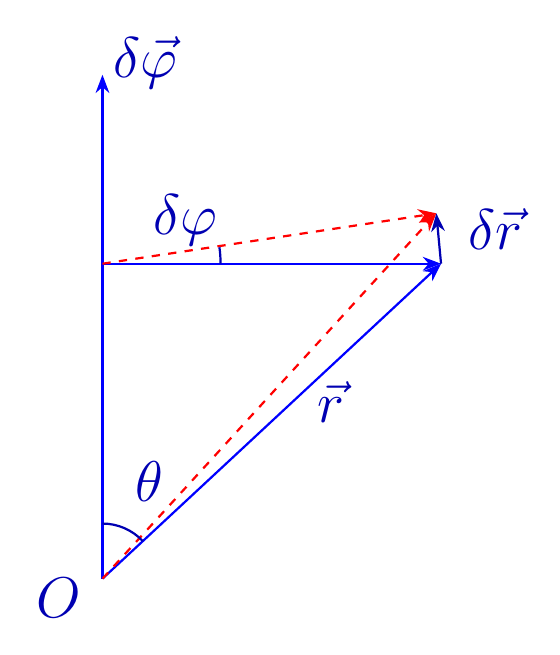
\begin{tikzpicture}[>=Stealth, thick, every node/.style={font=\fontsize{20}{24}\selectfont}]

  % ---- geometry -----------------------------------------------------
  \coordinate (O) at (0,0);
  \coordinate (A) at (0,4.0);
  \coordinate (Top) at (0,6.4);
  \coordinate (Q) at (4.3,4.0);
  \coordinate (Qp) at (4.24,4.64);

  % ---- vertical axis (red), labelled delta-phi-vector at the tip --------
  \draw[blue, ->] (O) -- (Top);
  \node[blue!70!black] at ($(Top)+(0.55,0.15)$) {$\delta\vec{\varphi}$};

  % ---- radius vector r (red), from O to Q --------------------------------
  \draw[blue, ->] (O) -- (Q);
  \node[blue!70!black] at ($(O)!0.56!(Q)+(0.5,0.)$) {$\vec{r}$};

\draw[red, dashed, ->] (O) -- (Qp);

  % ---- tangential reference segment (red), from A to Q -------------------
  \draw[blue, ->] (A) -- (Q);

  % ---- (r+dr)-direction reference (gray), from A to Qp --------------------
  \draw[red,dashed, ->] (A) -- (Qp);

  % ---- delta r vector (blue), from Q to Qp -------------------------------
  \draw[blue!70!black,->] (Q) -- (Qp);
  \node[blue!70!black] at ($(Qp)+(0.75,-0.2)$) {$\delta\vec{r}$};

  % ---- theta angle mark at O, between the vertical axis and r -----------
  \draw[blue!70!black] ({0.7*cos(43)},{0.7*sin(43)}) arc[start angle=43, end angle=90, radius=0.7];
  \node[blue!70!black] at (0.59,1.23) {$\theta$};

  % ---- delta-phi angle mark at A, between AQ and AQp ----------------------
  \draw[blue!70!black] ($(A)+(1.5,0)$) arc[start angle=0, end angle=8, radius=1.5];
  \node[blue!70!black] at ($(A)+(1.05,0.55)$) {$\delta\varphi$};

  % ---- point O label --------------------------------------------------
  \node[blue!70!black] at ($(O)+(-0.55,-0.25)$) {$O$};

\end{tikzpicture}
\end{document}
